\chapter{Sentimental Classification Model and Evaluation}
\section{Sentimental Data Exploration}
We obtained the sentimental classification datasets from \href{https://www.kaggle.com/datasets/smaheshacharya/nepali-sentiment-analysis}{Kaggle} and \href{https://huggingface.co/rockerritesh/NepaliSentiment/tree/main}{HuggingFace}. 
Some sample of the dataset were as follow:

\begin{figure}[H]
    \centering
    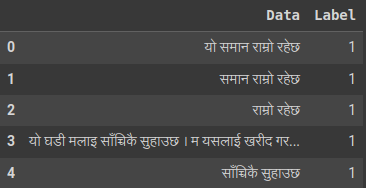
\includegraphics[scale = 0.7]{sentimental_classifier_model/data_format.png}
    \caption{Sentimental Classification Dataset}
    \label{fig:Sentimental Classification Dataset}
\end{figure}

Dataset obtained from kaggle and huggingface has 2186 and 7985 unique entries respectively. The dataset distribution of kaggle is as follow:



\begin{figure}[H]
    \centering
    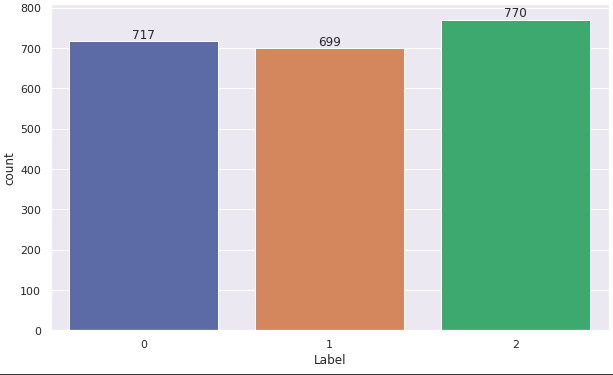
\includegraphics[scale = 0.5]{sentimental_classifier_model/partial_data.png}
    \caption{Kaggle Dataset Label Count plot}
    \label{fig:Kaggle Dataset Label Count plot}
\end{figure}

Both datasets were combined and the resulting data count plot is as follow:
\begin{figure}[H]
    \centering
    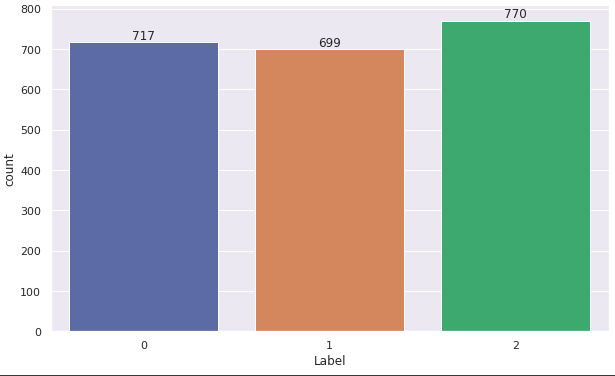
\includegraphics[scale = 0.5]{sentimental_classifier_model/all_data.png}
    \caption{Combined Dataset Label Count plot}
    \label{fig:Combined Dataset Label Count plot}
\end{figure}

\section{Data Preprocessing}
The text data of our dataset was preprocessed as follow:
\begin{enumerate}
    \item Tokenized the sentence using \textbf{nepalitokenizer}
    \item Removed the nepali stopwords. Stop words were obtained from \textbf{nltk.corpus.stopwords}
    \item Nepali words were stemmed using \textbf{nepali\_stemmer.stemmer.NepStemmer}
\end{enumerate}

\section{Train test split}
80\%, 10\% and 10\% of the datasets were used for training, validation and testing of the model.

\section{Tokenization and One Hot Encoding}
Tokenization was performed using \textbf{keras.preprocessing.text.Tokenizer} and padded using \textbf{keras\_preprocessing.sequence.pad\_sequences}. The UNIQUE\_WORD\_COUNT was selected to be 3179 and MAX\_PAD\_LENGTH =  10 with the help of following graph.

\begin{figure}[H]
    \centering
    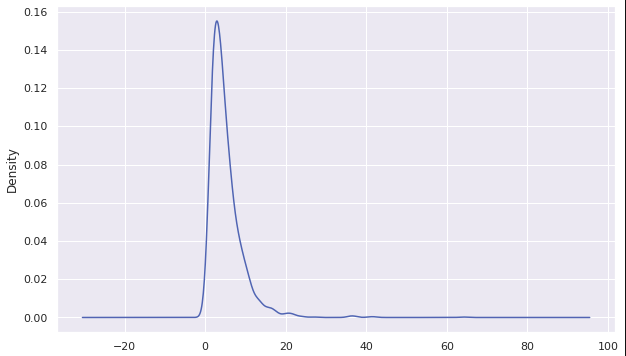
\includegraphics[scale = 0.55]{sentimental_classifier_model/length_count_plot.png}
    \caption{Length Series Count Plot : Length 10 seems to be appropriate for padding length from the plot.}
    \label{fig:Length Series Count Plot}
\end{figure}

\section{Sentimental Classification Model}
Only kaggle dataset was used for the training and evaluation of the classification model version 1 and version 2. 

\subsection{Sentimental Classification Model Version 1}
The summary of the sentimental classification version 1 is as follow:

\begin{figure}[H]
    \centering
    \includegraphics[scale = 0.5]{sentimental_classifier_model/v1/summary.png}
    \caption{Sentimental Model Version 1 Summary}
    \label{fig:Sentimental Model Version 1 Summary}
\end{figure}

The training and test loss and accuracy variation with epochs are shown below:

\begin{figure}[H]
    \centering
    \includegraphics[scale = 0.5]{sentimental_classifier_model/v1/acc.png}
    \caption{Sentimental Model Version 1 Accuracy Curve}
    \label{fig:Sentimental Model Version accuracy curve}
\end{figure}

\begin{figure}[H]
    \centering
    \includegraphics[scale = 0.5]{sentimental_classifier_model/v1/loss.png}
    \caption{Sentimental Model Version 1 Loss Curve}
    \label{fig:Sentimental Model Version 1 loss curve}
\end{figure}

The confusion matrix heatmap plot and classification report are shown below:


\begin{figure}[H]
    \centering
    \includegraphics[scale = 0.6]{sentimental_classifier_model/v1/cm.png}
    \caption{Sentimental Model Version 1 Confusion Matrix}
    \label{fig:Sentimental Model Version 1 Confusion Matrix}
\end{figure}

\begin{figure}[H]
    \centering
    \includegraphics[scale = 0.7]{sentimental_classifier_model/v1/cr.png}
    \caption{Sentimental Model Version 1 Classification Report}
    \label{fig:Sentimental Model Version 1 Classification Report}
\end{figure}

% Next Model version 2

\subsection{Sentimental Classification Model Version 2}
The summary of the sentimental classification version 2 is as follow:

\begin{figure}[H]
    \centering
    \includegraphics[scale = 0.5]{sentimental_classifier_model/v3/summary.png}
    \caption{Sentimental Model Version 2 Summary}
    \label{fig:Sentimental Model Version 2 Summary}
\end{figure}

The training and test loss and accuracy variation with epochs are shown below:

\begin{figure}[H]
    \centering
    \includegraphics[scale = 0.5]{sentimental_classifier_model/v3/acc.png}
    \caption{Sentimental Model Version 2 Accuracy Curve}
    \label{fig:Sentimental Model Version 2 accuracy curve}
\end{figure}

\begin{figure}[H]
    \centering
    \includegraphics[scale = 0.5]{sentimental_classifier_model/v3/loss.png}
    \caption{Sentimental Model Version 2 Loss Curve}
    \label{fig:Sentimental Model Version 2 loss curve}
\end{figure}

The confusion matrix heatmap plot and classification report are shown below:


\begin{figure}[H]
    \centering
    \includegraphics[scale = 0.6]{sentimental_classifier_model/v3/cm.png}
    \caption{Sentimental Model Version 2 Confusion Matrix}
    \label{fig:Sentimental Model Version 2 Confusion Matrix}
\end{figure}

\begin{figure}[H]
    \centering
    \includegraphics[scale = 0.7]{sentimental_classifier_model/v3/cr.png}
    \caption{Sentimental Model Version 2 Classification Report}
    \label{fig:Sentimental Model Version 2 Classification Report}
\end{figure}